\begin{figure}
  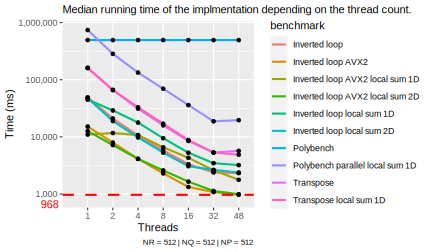
\includegraphics[scale=0.54]{Doitgen_OpenMP/classic_data_plot.eps}
  \caption{Comparisons of several implementations for Doitgen.}
  \label{fig:doitgen_openmp_classic_data}
\end{figure}

\begin{figure}
  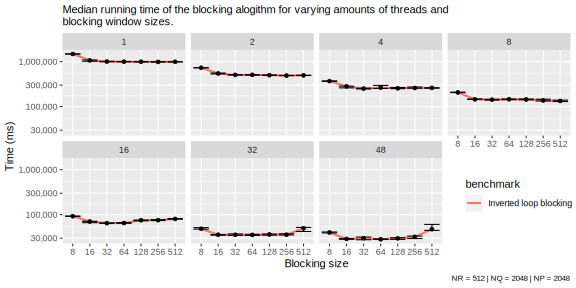
\includegraphics[scale=0.41]{Doitgen_OpenMP/blocking_data_scale_plot.eps}
  \caption{Study of the blocking algorithm with different parameters. Each plot corresponds to a specific number of threads.}
  \label{fig:doitgen_openmp_blocking_scale_data}
\end{figure}

\begin{figure}
  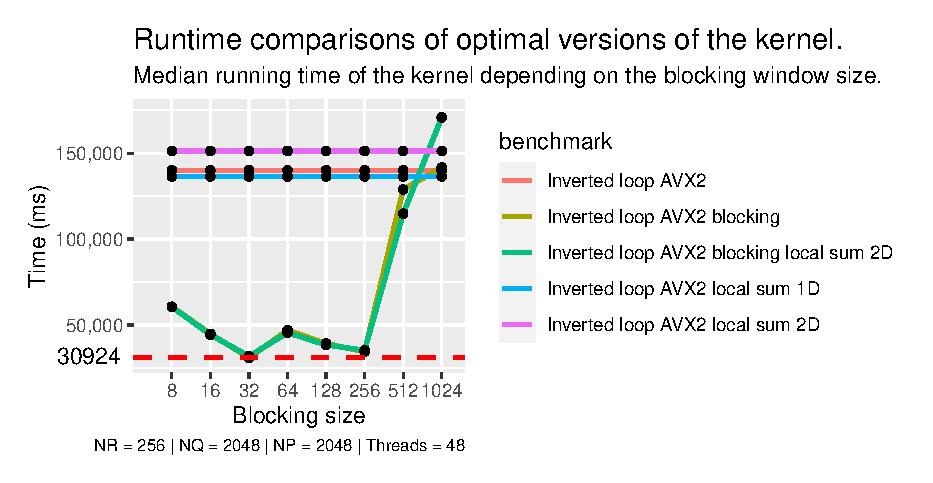
\includegraphics[scale=0.54]{Doitgen_OpenMP/optimized_data_plot.eps}
  \caption{The dashed line represents the smallest running time.}
  \label{fig:doitgen_openmp_optimized_data}
\end{figure}

\begin{figure}
  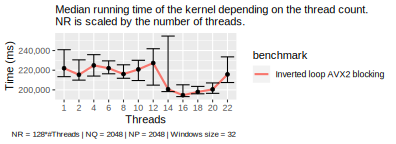
\includegraphics[scale=0.59]{Doitgen_OpenMP/scaling_data_plot.eps}
  \caption{Study of the inverted loop AVX2 blocking implementation with scaling.}
  \label{fig:doitgen_openmp_scaled_data}
\end{figure}

\subsubsection{Proposed methods}\label{proposed_methods_openmp}

In this section, we will talk about the parallelization and optimization of the doitgen kernel using the Open\hyp{}MP API. We parallelized Doitgen as follows : one thread computes a sequence of \textbf{complete} matrix-matrix multiplications. More concretely, the parallelism occurs along the NR axis of the input matrix. To extract the most performance out of our CPU, we need to leverage the cache. To explore the impact of better cache utilization, we implemented a version of the algorithm that uses a transposed C4 matrix, a version where the two inner loops are inverted and a blocking version.

\mypar{Local sum} The initial version of the kernel provided by Polybench does not use an input and output matrix, only an input matrix is used. Then, in the kernel, the elements of a resulting line are incrementally built up and stored into an array that is then put back in the input matrix.
This way of performing the computation consumes $\NR\times\NQ\times\NP + \NP$ memory rather than $2\times\NR\times\NQ\times\NP$ when an output matrix is used. The difference between the versions with a local sum array and without will be explored in the following section.
Also, in the parallel algorithms, each thread has its own sum array, resulting in a ${\rm\#Threads}\times\NP$ table when a 1D sum array is used and in a ${\rm\#Threads}\times\NQ\times\NP$ table when a 2D sum array is used.

\mypar{Transpose version} In this version, the C4 matrix is transposed, it is thus traversed row by row.

\mypar{Inverted loops version} We incrementally build the elements of a line of the output matrix by traversing A by rows and C4 by rows. Then, we switch to another line of C and another line of A to build the elements of another line of the output matrix.

\mypar{Blocking version} In the blocking version of the kernel, the goal is to reuse values brought in from cache as much as possible. This is achieved by multiplying sub-matrices rather than multiply one matrix with another at once. This improvement can be combined with one of the two mentioned previously. As currently implemented, this version only works if the blocking size divides the matrix size.

\mypar{Vectorization}
The vectorization version of the kernel uses the AVX2 and FMA instruction sets. The AVX2 instruction set deals with 256 bits registers, allowing us to load doubles (8 bytes) 4 by 4. As currently implemented, this version only works if the matrix row size is divisible by 4.

\subsubsection{Experimental results}\label{experimental_results_openmp}
Here, results of the benchmarking of the different implementations will be presented.

\mypar{Finding the best implementation}
First, we decided to benchmark all the implementations with a rather small matrix size to see what the fastest were. See Figure \ref{fig:doitgen_openmp_classic_data} (beware of the logarithmic scale). We clearly see that the inverted loop AVX2 implementations are the fastest ones.

\mypar{Blocking window size}
Now, we want to know if pursuing blocking is worth it and how it performs under different blocking window sizes and varying amounts of threads. The results are available in Figure \ref{fig:doitgen_openmp_blocking_scale_data}. We see that the higher the thread count the higher the impact of blocking on performance. This may be because this allows for threads to work on different parts of the matrix, causing less cache coherency traffic and less cache associativity issues.

\mypar{Finding the best version}
With this data we can now conclude that an inverted loop AVX2 implementation with blocking should yield the best results. The outcome of this experiment is available in Figure \ref{fig:doitgen_openmp_optimized_data}.
Blocking improves greatly the performance of the algorithm. It seems to have a greater impact than on single threaded applications. The benchmarks appearing on the figure that do not use blocking were not run for each blocking size, they should be read as constant straight lines. Also, the 1D local sum version seems to be faster than the other two. This may be explained by cache coherency traffic, cache associativity and lower memory consumption. In Figure ~\ref{fig:doitgen_openmp_scaled_data}\footnote{We didn't manage to plot for greater thread counts(the limit is 22) because of memory consumption issues.}, the running time varies around 220s for different amounts of threads. This may be because the chosen window size is tailored to work well with 48 threads but not necessarily for other thread counts.